%========================================================================================%
%					NOTE
%========================================================================================%
% Probably this theme will not compile with standard pdftolatex compiler due to lack of some 
% fonts used in the theme. It is recommended to compile with XeLaTex instead.

% !TEX program = xelatex

%========================================================================================%
%					DOCUMENT SETUP
%========================================================================================%
\documentclass[10pt]{beamer} 
\usetheme[progressbar=frametitle]{metropolis}

\usepackage{textpos}


%For making diagram and drawing
\usepackage{tikz}
\usetikzlibrary{shapes,arrows, fit, positioning}

%For appendix
\usepackage{appendixnumberbeamer}


\usepackage[export]{adjustbox}

%Some additional graphcs tools
%\usepackage{graphicx}
%\usepackage{datatool}
%\usepackage{animate}

% For someone using the pgfplot tools
%\usepackage{pgfplots}
%\usepgfplotslibrary{dateplot, groupplots}
%\pgfplotsset{compat=1.14}
%\usepgfplotslibrary{fillbetween}

%Remove words break, wrap instead
\usepackage[none]{hyphenat}


%for custom date
%\usepackage[english]{babel}
\usepackage[polish,main=english]{babel}
\usepackage[utf8]{inputenc}
\usepackage[nodayofweek,level]{datetime}

\usepackage{xspace}
\newcommand{\themename}{\textbf{\textsc{metropolis}}\xspace}


%========================================================================================%
%	ADDITIONAL SETUP - added by GG
%========================================================================================%
\usepackage{csquotes}
\usepackage{bm} %bold in math mode
\usepackage{bbold} % math 1 - identity matrix
\usepackage{amsmath, amsthm, amsfonts, amssymb}
\usepackage{bbm}

\usepackage{caption}
\usepackage{graphicx, subfigure}
% \usepackage[compatibility=false]{caption}
% \usepackage{subcaption}
% \usepackage{floatrow}

\usepackage{multicol}
\usepackage{lipsum}


\usepackage[
style=numeric, % Citation Style
%style=verbose-trad2, % Citation Style
%backend=biber,
backend=bibtex,
%natbib=true
]{biblatex}
%\usepackage[style=authoryear, backend=biber]{biblatex}
\renewbibmacro{in:}{} % suppress the "In: " before the journaltitle

\hypersetup{
urlcolor=mDarkTeal, 
linkcolor=mDarkTeal, % internal links
citecolor=mDarkTeal, % citations
urlcolor=mDarkTeal, % external links/urls
colorlinks=true
} % Colors hyperlinks in blue - change to black if annoying
\addbibresource{library.bib}

\usepackage{cleveref}  % Warning: cleverref has to be loaded after hyperref!
% shortcuts from ŁŁW
\newcommand{\pr}[1]{\frac{\partial}{\partial #1}}
\newcommand{\rr}[2]{\frac{\partial #1}{\partial #2}}
\newcommand{\ppr}[1]{\frac{\partial^2}{\partial #1^2}}
\newcommand{\prr}[2]{\frac{\partial^2}{\partial #1\partial #2}}
\newcommand{\rpr}[2]{\frac{\partial^2 #1}{\partial #2^2}}
\newcommand{\rrr}[3]{\frac{\partial^2 #1}{\partial #2\partial #3}}

\newcommand{\R}{\mathbb{R}}
\newcommand{\E}{\mathbb{E}}
\newcommand{\Var}{\text{Var}}
\newcommand{\eq}{\text{eq}}
%\newcommand{\x}{\overline{x}}
\newcommand{\f}{\tilde{f}}
%===================================================================================%
%				FRONT PAGE
%===================================================================================%
\titlegraphic{%
\hfill%

\includegraphics[height=1.5cm, valign=c]{logos/Logo_icm_niebieskie.png}%
\hspace{15pt}%

\includegraphics[height=1.5cm, valign=c]{logos/ccfd3.png}%
\hspace{15pt}%

\includegraphics[height=1.5cm, valign=c]{logos/symbol-PL.pdf}%
}

\author{\underline{Grzegorz Gruszczyński}$^{a,b}$, Łukasz Łaniewski-Wołłk$^b$} 

\title{Application of the Cascaded Lattice Boltzmann Method with 
interpolated boundary conditions to heat transfer problems}

\institute
{
\textbf{$^a$University of Warsaw, Interdisciplinary Centre for Mathematical and Computational Modelling\newline} %\\[1em] 
\textbf{$^b$Warsaw University of Technology, Faculty of Power and Aeronautical Engineering}
%\texttt{e-mail address}
}

%\date{\vspace{5pt}\today}
\date{\vspace{5pt}\formatdate{13}{2}{2019}}

%===================================================================================%
%				THEME COLORS
%===================================================================================%
% specify main colors which are being used by the theme
\definecolor{bordercolor}{HTML}{002699}
\definecolor{fillcolor}{HTML}{002699}

% fix theme black color which affects tikz plots
\definecolor{black}{RGB}{0,0,0}




%===================================================================================%
%				ACTUAL DOCUMENT CONTENT
%===================================================================================%

\begin{document}

\maketitle

%force to add logs to the each frame title
\addtobeamertemplate{frametitle}{}{%
\begin{textblock*}{100mm}(.835\textwidth, -0.9cm)
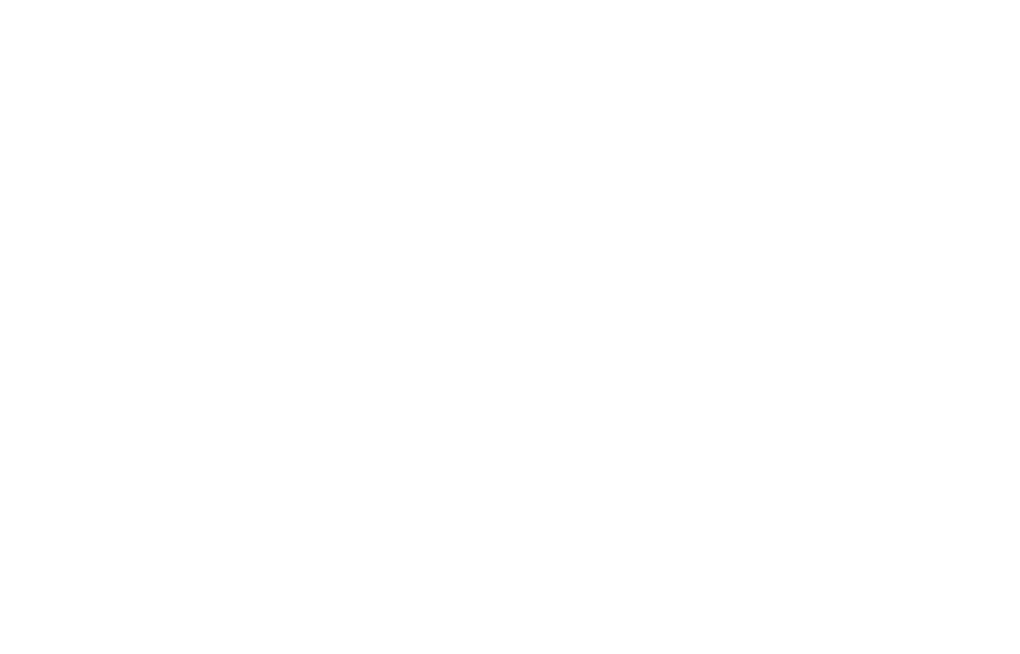
\includegraphics[height=0.8cm, valign=c]{logos/Logo_icm_biale.png}\hspace{9pt}
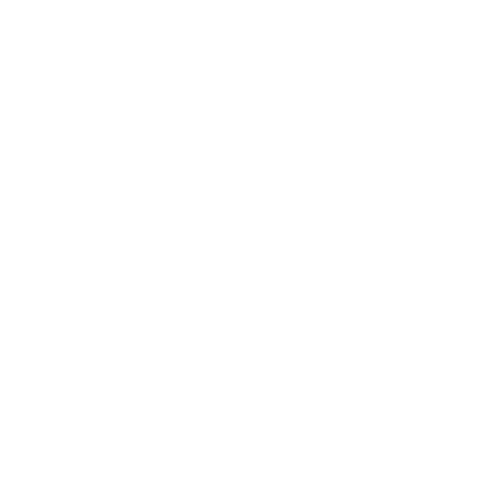
\includegraphics[height=0.8cm, valign=c]{logos/ccfd3_white.png}\hspace{9pt}
%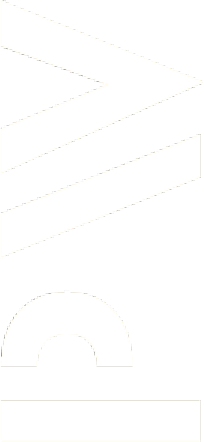
\includegraphics[height=0.78cm, valign=c]{logos/symbol-PL-white.pdf}
\end{textblock*}}

\begin{frame}\frametitle{Table of contents}
\tableofcontents
\end{frame} 

\section{Introduction} 
\subsection{Problem Statement and Governing Equations} 
\begin{frame}\frametitle{Governing Equations} 
%We simulate an incompressible flow coupled with heat transfer across solid-fluid interface. \newline
\metroset{block=fill}
\begin{exampleblock}{Goal}
Simulate an incompressible flow coupled with heat transfer problem. \newline
\end{exampleblock}
  
The continuity and momentum equations are:
\begin{eqnarray}  
\left\{
	\begin{array}{ll}
\frac{\partial \rho}{\partial t} + \nabla \cdot \rho \textbf{u} = 0 \\
\rho\left( \frac{\partial \textbf{u} }{\partial t} + \textbf{u} \cdot \nabla \textbf{u}\right) = -\nabla p + \nabla \cdot (\mu[ \nabla \textbf{u} + (\nabla \textbf{u})^\top]) + \textbf{F}
	\end{array}\nonumber 
\right.
\end{eqnarray}

The Enthalpy balance equation is:
\begin{align}
\pr{t} (\rho c_p T ) + \nabla \cdot (\boldsymbol{u} \rho c_p T ) &= \nabla \cdot (k \nabla T)  + \dot{q} \nonumber %\label{eq:enthalpy_transfer_eq}
\end{align}
\end{frame}


\begin{frame}[standout]
    Lattice Boltzmann Method
\end{frame}

\subsection{LBM - Theory}
\begin{frame}\frametitle{The Lattice Boltzmann equation}
Probability of finding a particle in the phase space:
\begin{figure}
  \begin{minipage}[c]{0.6\textwidth}
    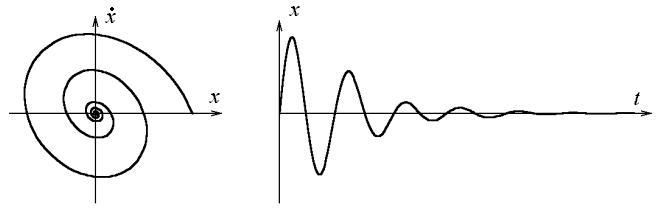
\includegraphics[width=\textwidth]{obrazki/PhaseSpace.png} 
  \end{minipage}\hfill
  \begin{minipage}[c]{0.4\textwidth} % use [c], [t] or [b] for vertical alignment
    \caption{$\Psi = \Psi(t, \textbf{x}, \dot{\textbf{x}}$)} \label{fig:PhaseSpace}
  \end{minipage}
\end{figure}

\pause
In an infinitesimally small volume of the phase space $d\textbf{x} d\textbf{u} $:
\begin{eqnarray} 
	 \Psi_{no\,collisions}(t +dt, \textbf{x} + d\textbf{x}, \textbf{u} + d\textbf{u}) d\textbf{x} d\textbf{u} =
	 \Psi_{no\,collisions}(t, \textbf{x}, \textbf{u}) d\textbf{x} d\textbf{u}\nonumber
\end{eqnarray}

\pause
Now, include the collision term  $\mathbb{C}(\Psi)$:
\begin{eqnarray} \label{distributionFunctionEvolution}
	 \Psi(t +dt, \textbf{x} + d\textbf{x}, \textbf{u} + d\textbf{u})  d\textbf{x} d\textbf{u}=
	 \Psi(t, \textbf{x}, \textbf{u}) d\textbf{x} d\textbf{u} + \mathbb{C}(\Psi)  d\textbf{x} d\textbf{u} dt  \nonumber
\end{eqnarray} 
\end{frame} 

\begin{frame}\frametitle{The Lattice Boltzmann equation}

Taylor series expansion:
\begin{eqnarray} 
	 \Psi(t +dt, \textbf{x} + d\textbf{x}, \textbf{u} + d\textbf{u}) =
	 \Psi(t, \textbf{x}, \textbf{u}) + \frac{\partial \Psi}{\partial t} dt + 
	 \nabla_{\textbf{x}}\Psi d\textbf{x} +
	 \nabla_{\textbf{u}}\Psi d\textbf{u} \nonumber
\end{eqnarray}

\pause
Plug in:
\makebox[\linewidth]{\parbox{12.8cm}{
\begin{eqnarray} 
	\left[  \Psi(t, \textbf{x}, \textbf{u}) +
	 \frac{\partial \Psi}{\partial t} dt + 
	 \nabla_{\textbf{x}}\Psi d\textbf{x} +
	 \nabla_{\textbf{u}}\Psi d\textbf{u} \right] d\textbf{x} d\textbf{u} 
	 = \bigg[ \Psi(t, \textbf{x}, \textbf{u}) + \mathbb{C}(\Psi) dt \bigg] d\textbf{x} d\textbf{u} \nonumber 
\end{eqnarray}
}}

\pause
Reformulate velocity $ \textbf{u} = \frac{d\textbf{x} }{dt}$ and acceleration 
$ \frac{d \textbf{u}}{dt} =  \frac{\textbf{F}}{\rho}$:
\begin{eqnarray} \label{Boltzmann_equation_withForce}
	\dfrac{\partial \Psi}{\partial t} + (\textbf{u} \cdot \nabla_{\textbf{x}}) \Psi +
	 (\frac{\textbf{F}}{\rho} \cdot \nabla_{\textbf{u}}) \Psi 
	 = \mathbb{C}(\Psi) \nonumber
\end{eqnarray}
%The Boltzmann equation can be viewed as a substantial derivative (of an intensive quantity $\Psi$) which is equal to the collision term $ \mathbb{C}$ applied to the distribution function of $\Psi$.
\end{frame} 

\begin{frame}\frametitle{Lattice Boltzmann equation - Summary}
Streaming and Collision:
\begin{eqnarray}
	 \underbrace{ \Psi(t +dt, \textbf{x} + d\textbf{x}, \textbf{u} + d\textbf{u})  d\textbf{x} d\textbf{u} }_{Streaming}=
	 \underbrace{\Psi(t, \textbf{x}, \textbf{u}) d\textbf{x} d\textbf{u} + \mathbb{C}(\Psi)  d\textbf{x} d\textbf{u} dt}_{Collision}  \nonumber
\end{eqnarray} 

The Boltzmann equation can be viewed as a substantial derivative (of an intensive quantity $\Psi$) which is equal to the collision term $ \mathbb{C}$ applied to the distribution function of $\Psi$:
\begin{eqnarray}
	\dfrac{\partial \Psi}{\partial t} + (\textbf{u} \cdot \nabla_{\textbf{x}}) \Psi +
	 (\frac{\textbf{F}}{\rho} \cdot \nabla_{\textbf{u}}) \Psi 
	 = \mathbb{C}(\Psi) \nonumber
\end{eqnarray}
\end{frame}

\subsection{Discrete Boltzmann equation}
\begin{frame}\frametitle{Discretization of the Lattice Boltzmann equation}
\pause
\begin{eqnarray} 
  \underbrace{ f_i(\bm{x} + \bm{e_i} \Delta {\bm{x}}, t +  \Delta {t} ) }_{Streaming} =
  \underbrace{ f_i(\bm{x}, t ) - \frac{1}{\tau } ( f_i - f_i^{eq}) + F_i(\bm{x}, t ) }_{Collision} \nonumber
\end{eqnarray}
\begin{itemize}
\item  $\tau = \tau(\nu)$ relaxation parameter, $\nu$ is the kinematic viscosity 
\item $f_i$ - discrete probability distribution function
\item $F_i$ - source term (ex. gravity force)
\end{itemize}
\begin{figure}
  \begin{minipage}[c]{0.6\textwidth}
    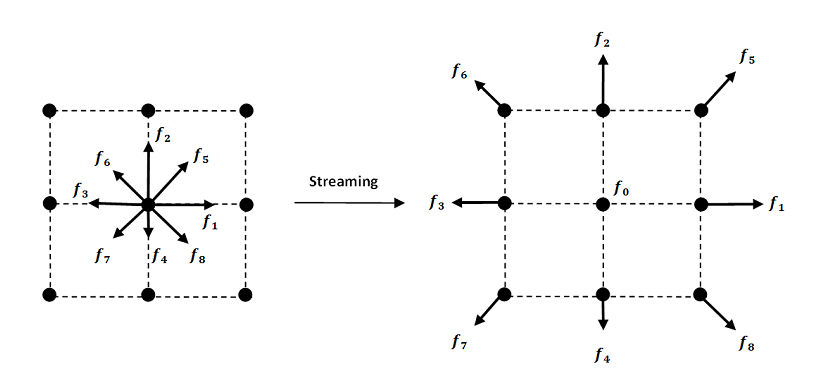
\includegraphics[width=\textwidth]{obrazki/streaming.png} 
  \end{minipage}\hfill
  \begin{minipage}[c]{0.4\textwidth} % use [c], [t] or [b] for vertical alignment
    \caption{D2Q9: Streaming} \label{fig:Streaming}
  \end{minipage}
\end{figure}
\end{frame} 

\subsection{LBM - Algorithm}
\begin{frame}[plain] \frametitle{Algorithm: Fluid} 
\textit{1} Initialize $ \enspace f_i ^{in} $ \\ \vspace{2.5em}

\pause 
\textit{2} Compute 
$ \rho = \sum_{i=0}^{8} f_i ^{in}(\boldsymbol{x},t)
          \hspace{2 em}  and  \hspace{2 em}
      	 \boldsymbol{u}(\boldsymbol{x},t) = \frac{1}{\rho} \sum_{i=0}^{8} \, f_i ^{in}(\boldsymbol{x},t) \boldsymbol{e}_i +  \frac{\textbf{F}}{2 \rho} \delta t 
      	 $ \\ \vspace{2.5em}

\pause
\textit{3} Compute 
$  f_i ^{eq}(\boldsymbol{x},t) =  w_i \rho 
 \left[ 1 + \frac{\boldsymbol{e}_i \boldsymbol{u}}{c_s^2 e^2} + \frac{ (\boldsymbol{e}_i \boldsymbol{u})^2}{2 c_s^4 e^4} - \frac{\boldsymbol{u}^2 } {2c_s^2 e^2} \right] $  where $c_s^2 = \frac{1}{3}$
 \\ \vspace{2.5em}

\pause 
\textit{4} Collision  
$  f_i ^{out}(\boldsymbol{x},t) = f_i^{in}(\boldsymbol{x},t) - \frac{1}{\tau_f} \bigg[ f_i^{in}(\boldsymbol{x},t) - f_i^{eq}(\boldsymbol{x},t) \bigg] + F_i(\bm{x}, t ) $ \\ \vspace{2.5em}

\pause
\textit{5} Streaming 
$  f_i ^{in}(\boldsymbol{x} + \boldsymbol{e}_i ,t+1) =  f_i^{out} (\boldsymbol{x},t) $ 

\end{frame} 

\section{Heat Transfer in LBM}
\subsection{Fixed Prandl Number problem}
\begin{frame}\frametitle{Macroscopic variables}
Macroscopic variables can be recovered from the moments of DF:
\begin{align*}  
\textit{mass density: \hspace{1em}} \rho &= \int f(\boldsymbol{x} , \boldsymbol{\xi}, t, T) d^3 \xi \\
\textit{momentum density: \hspace{1em}} \rho \boldsymbol{u} &= \int  \boldsymbol{\xi} f(\boldsymbol{x} , \boldsymbol{\xi}, t, T) d^3 \xi \\
\textit{internal energy density: \hspace{1em}} \rho i&= \dfrac{1}{2} \int |\boldsymbol{\xi} - \boldsymbol{u}|^2 f(\boldsymbol{x} , \boldsymbol{\xi}, t, T) d^3 \xi
\end{align*}

Why \underline{not} extract the temperature from the internal energy as $i=c_v T$ ?

\pause
Such approach together with the SRT collision operator would lead to the \textit{fixed Prandl Number problem}, 
because thermal conductivity can not be tuned independently of kinematic viscosity. % \parencite{He1998a,Cercignani1988}.

\end{frame}

\begin{frame}\frametitle{Fixed Prandl Number problem}
The are three approaches to solve the issue:
\begin{enumerate}
\item Multi Relaxation Time + Multispeed LBM (there are not enough moments on standard lattices). 
\item Introduce new distribution function, which can evolve in its own way, responsible for the energy field. 
\item Use LBM for hydrodynamic coupled with another solver (e.g. finite difference) for temperature field.
\end{enumerate}
\end{frame}


\begin{frame}[plain]\frametitle{Algorithm: Energy Field}
`Advection - Diffusion` of  $H$ is solved on a separate D2Q9 lattice 
\\ \vspace{1.5em}

\textit{1} Initialize 
$ h_i ^{in} (\boldsymbol{x},t) $ \\ \vspace{2.5em}
%\pause

\textit{2} Compute 
$  H = \sum_{i=0}^{9} h_i ^{in}(\boldsymbol{x},t) $ \\ \vspace{2.5em}

%\pause
\textit{3} Compute 
$ h_i ^{eq}(\boldsymbol{x},t) = H w_i  
\left[ 1 + \frac{\boldsymbol{e}_i \boldsymbol{u}}{c_s^2 e^2} + \frac{ (\boldsymbol{e}_i \boldsymbol{u})^2}{2 c_s^2 e^4} - \frac{\boldsymbol{u}^2 } {2c_s^2 e^2} \right]  $  \\ \vspace{2.5em}
 
%\pause
\textit{4} Collision 
$ h_i ^{out}(\boldsymbol{x},t) = h_i^{in}(\boldsymbol{x},t) - \frac{1}{\tau_T} \bigg[ h_i^{in}(\boldsymbol{x},t) - h_i^{eq}(\boldsymbol{x},t) \bigg] + \dfrac{\dot{q}}{\rho c_p}$ \\ \vspace{2.5em}

\textit{5} Streaming 
$  h_i ^{in}(\boldsymbol{x} + \boldsymbol{e}_i ,t+1) =  h_i^{out} (\boldsymbol{x},t) $ \\ \vspace{2.5em}

\end{frame} 

\begin{frame}\frametitle{Result}
Now, the temperature field can be solved in a fluid:

\begin{center}
%{\huge ? }
\begin{figure}
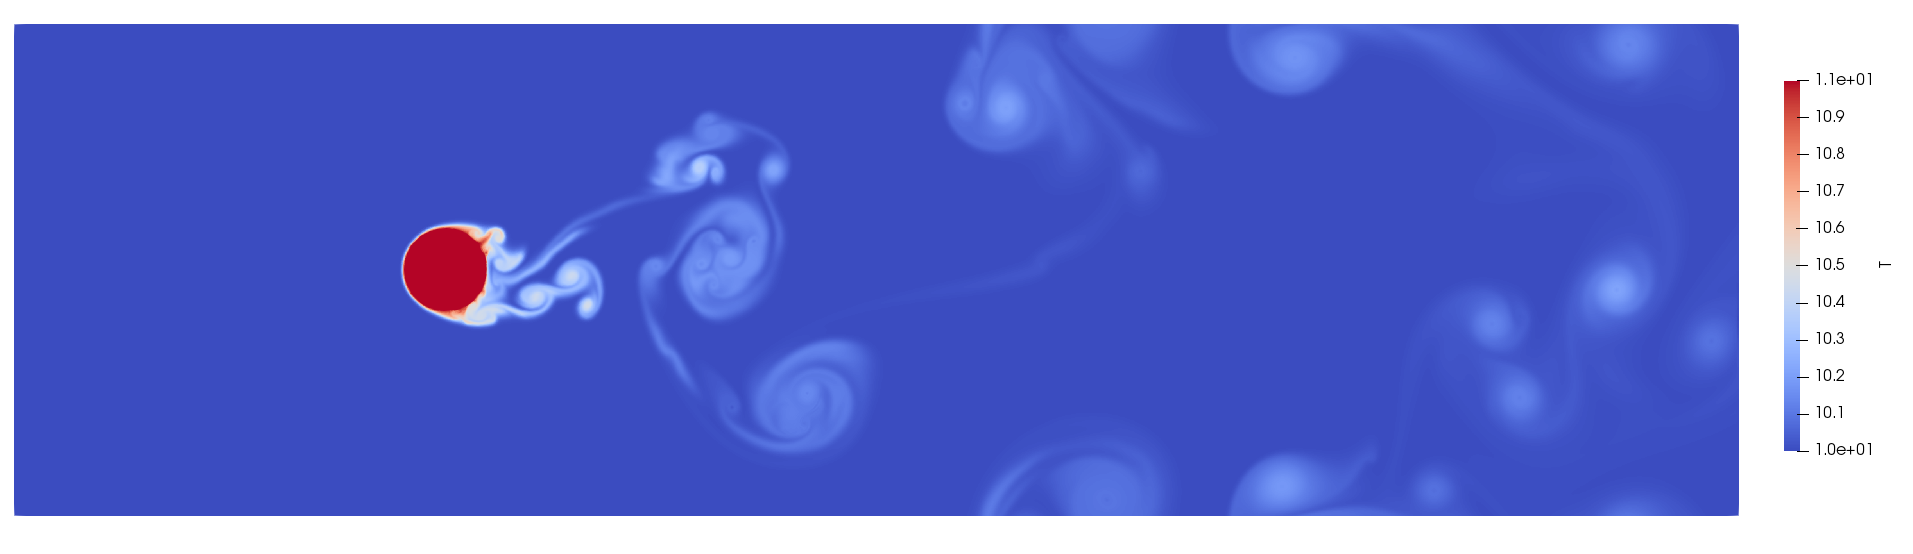
\includegraphics[width = \textwidth]{obrazki/HotKarman_Re1000.png} 
% HotKarman_Re1000_D0_1.28e+02_nu_0.0055_U_4.30e-02_bc_HeaterDirichletTemperatureEQ_CM_HIGHER
\caption{Re = 1000, Pr = 0.71, D = 128 [lu]}
\end{figure}
\end{center}
\end{frame}


\begin{frame}\frametitle{(De)Coupling of N-S and Energy equations}
Physically, equations are coupled:
\begin{itemize}
\item Energy Eq. $ \rightarrow $ NS: equation of state $f(p,\rho,T) = 0 $. \newline 
Usually, ideal gas $p(\rho, T) = \rho R T = \rho c_s^2 $ is assumed for single phase LBM models.
\item NS $ \rightarrow $ Energy Eq.: kinetic energy + dissipation (viscous heating) and compression work.
\end{itemize}
\pause
In simplified models, the NS equation is decoupled from energy eq.
The equation of state has a constant temperature $p(\rho, T) = \rho c_s^2 = \rho R T_0 $ and the sound speed is fixed as $c_s = \sqrt{R T_0}$ . \linebreak
As a result, these models are incompressible. \newline
To account for thermal advection the Boussinesq approximation can be employed,
\begin{align*} 
\rho(T) & \approx \rho_0 (1- \alpha_V (T-T_0)), \\
\boldsymbol{F}_{bouyancy} &= [\rho(T) - \rho_0] \boldsymbol{g} = - \boldsymbol{g} \rho_0 \alpha_V (T-T_0).
\end{align*} 
\end{frame}


\section{Theory - deeper dive}
\begin{frame}[standout]
    (Central) Moments
\end{frame}
\begin{frame}[plain]\frametitle{'Statistical' refreshment}

%\begin{multicols}{2}
\begin{figure}[H]
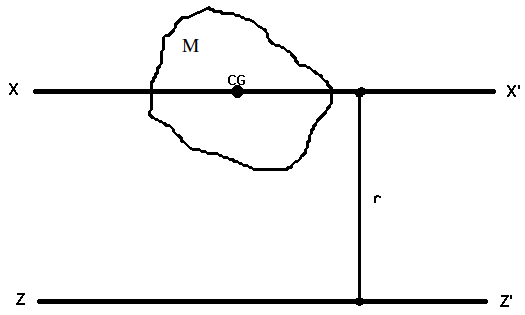
\includegraphics[width = 0.5 \textwidth]{obrazki/ParallelaxesTheory.png} 
%\caption{MRT: components of hydrodynamic forces}
\end{figure}
%\columnbreak 
\pause
\begin{eqnarray}\nonumber
m_0 &=& M = \int r^0 \rho(r) d \Omega \\ \nonumber
m_1 &=& \mu = \frac{1}{M}\int r^1 \rho(r) d \Omega \\ \nonumber
m_2 &=& I_{zz'} = \int r^2 \rho(r) d \Omega \\ \nonumber
\sigma ^2 &=&  I_{xx'}\int (r - \mu)^2 \rho(r) d \Omega \nonumber 
\end{eqnarray}
%\end{multicols}

\end{frame}

\begin{frame}[plain]\frametitle{Moments}
The raw moments and central moments:
\begin{eqnarray}
\kappa_{mn} &=& \sum_{i}(e_{i, x})^m ( e_{i, y})^n f_{i} \nonumber \label{eq:raw_mom_def} \\
\tilde{\kappa}_{mn} &=& \sum_{i} ( e_{i, x} - u_x)^m ( e_{i, y} - u_y)^n f_{i} \nonumber \label{eq:cm_mom_def}
\end{eqnarray}
\pause
Physical interpretation:
\begin{eqnarray} 
\rho &=& \kappa_{00} = \sum_i f_i \nonumber % \hspace{2em} \text{- normalized pressure} 
 \\
\rho \textbf{u} &=& [u_x, u_y]^\top = [ \kappa_{10}, \kappa_{01}]^\top 
= \sum_i f_i \textbf{e}_i + \frac{\textbf{F}}{2} \delta t \nonumber 
% \hspace{2em} \text{- macroscopic velocity} 
\end{eqnarray}

  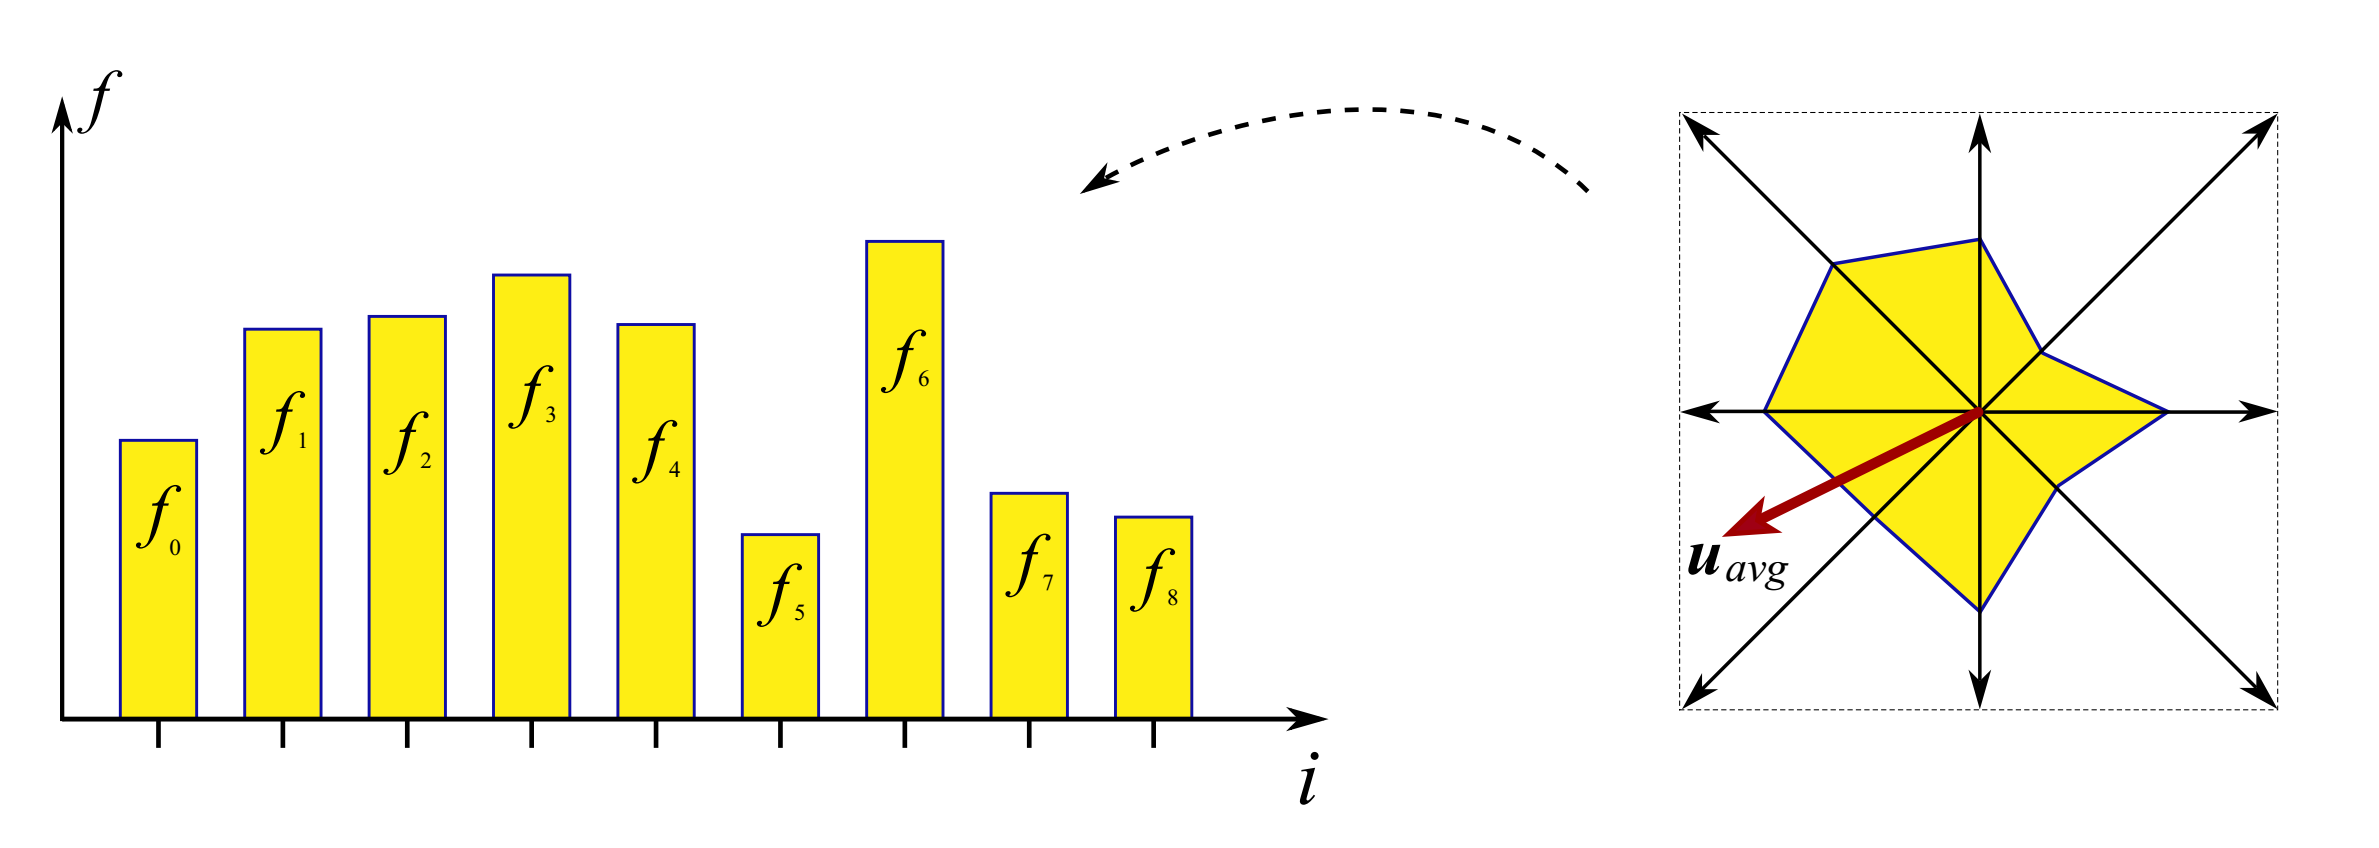
\includegraphics[width = 0.8 \textwidth]
   {obrazki/latticeVelocities_concept.png} 
\end{frame}

\begin{frame}\frametitle{Multiple Relaxation Time}
%\pause
Alternatively, moments can be expressed in terms of matrix transformations:
\begin{eqnarray}
\boldsymbol{\Upsilon} = \mathbbm{M} \boldsymbol{f} \nonumber \\
\boldsymbol{\tilde{\Upsilon}}= \mathbbm{N} \boldsymbol{\Upsilon} \nonumber
\end{eqnarray}
The resulting order of central moments is:
\begin{eqnarray} 
\boldsymbol{\tilde{\Upsilon}} = [
\tilde{\kappa}_{00}, 
\tilde{\kappa}_{10}, 
\tilde{\kappa}_{01}, 
\tilde{\kappa}_{20}, 
\tilde{\kappa}_{02}, 
\tilde{\kappa}_{11}, 
\tilde{\kappa}_{21}, 
\tilde{\kappa}_{12}, 
\tilde{\kappa}_{22}]^\top \nonumber
\end{eqnarray} 
\end{frame}

\begin{frame}\frametitle{Equilibrium distribution function}
The Maxwell-Boltzmann equilibrium distribution function in a continuous velocity space is known as:
\begin{eqnarray}  
\Psi^{\textit{M-B, eq}} = 
\Psi^{\textit{M-B, eq}}(\phi, \boldsymbol{\xi}, \boldsymbol{u}) =
\dfrac{\phi}{(2 \pi c_s^2)^{D/2}} 
exp \left[
-\frac{(\boldsymbol{\xi}-\boldsymbol{u})^2}{2 c_s^2}
\right] \nonumber \label{eq:Maxwellian}
\end{eqnarray}
where: 
\begin{eqnarray}
\phi  \hspace{3em} &-& \text{quantity of interest} \nonumber \\
\boldsymbol{\xi} \hspace{3em} &-& \text{microscopic `particle` velocity} \nonumber \\
\boldsymbol{u} \hspace{3em} &-& \text{macroscopic `flow` velocity} \nonumber
\end{eqnarray} 
%Where D is the number of dimensions. \newline
The continuous definition of the central moments is:
\begin{eqnarray}  
\tilde{\kappa}_{mn} = \int_{-\infty}^{\infty} \int_{-\infty}^{\infty} 
(\xi_x - u_x)^m (\xi_y -u_y)^n
\Psi(\phi, \boldsymbol{\xi}, \boldsymbol{u}) 
d \xi_x d \xi_y \nonumber \label{eq:cont_cm_mom_def}
\end{eqnarray}
\end{frame}

\begin{frame}[plain] \frametitle{Algorithm fluid - revisited} 
\textit{1} Initialize $ \enspace f_i ^{in} $ \\ \vspace{2.em}

%\pause
\textit{2} Compute 
$\textbf{u} = [u_x, u_y]^\top = [ \kappa_{10}, \kappa_{01}]^\top 
= \frac{1}{\rho}\sum_i f_i \textbf{e}_i + \frac{\textbf{F}}{2 \rho} \delta t \nonumber  $ \\ \vspace{2.em}
%\pause
\textit{3} Compute \linebreak
$\boldsymbol{\tilde{\Upsilon}}(\boldsymbol{x},t)
=\mathbbm{N}\mathbbm{M}\textbf{f}(\boldsymbol{x},t)$, \linebreak
%\hspace{1em}
%$\boldsymbol{\tilde{\Upsilon}}^{eq}(\boldsymbol{x},t)=$..., \hspace{1em} 
%$\tilde{\textbf{F}}(\boldsymbol{x},t)=$... 
$\boldsymbol{\tilde{\Upsilon}}^{eq} =
    [\rho, 
     0,  
     0, 
     c_s^2 \rho, 
     c_s^2 \rho, 
     0, 
     0, 
     0, 
     c_s^4 \rho] ^\top \nonumber  
$
$\tilde{\boldsymbol{F}}  = 
[
     0, 
     F_x /\rho , 
     F_y /\rho , 
     0, 
     0, 
     0, 
     c_s^2 F_y /\rho , 
     c_s^2 F_x /\rho , 
     0]^\top \nonumber 
$
\\ \vspace{2.em}
 
%\pause
\textit{4} Collision  %\linebreak
$  \boldsymbol{\tilde{\Upsilon}}(\textbf{x}, t + \delta t ) = 
\boldsymbol{\tilde{\Upsilon}} 
- \mathbbm{S} (\boldsymbol{\tilde{\Upsilon}} - \boldsymbol{\tilde{\Upsilon}}^{eq})
+ (\mathbbm{1} - \mathbbm{S}/2)\tilde{\textbf{F}} $ \\ \vspace{2.em}

%\pause
\textit{5} Streaming 
$  f_i(\textbf{x} + \textbf{e}\delta t, t + \delta t ) 
 =  
\mathbbm{M}^{-1} \mathbbm{N}^{-1} \boldsymbol{\tilde{\Upsilon}}_{i}(\textbf{x}, t + \delta t )  $ 
\end{frame} 

\section{(Un)structured Mesh}
%\begin{frame}[standout]
%(Un)structured Mesh?
%\end{frame}

\begin{frame}\frametitle{(Un)structured Mesh?}
\begin{center}
%{\huge ? }
\begin{figure}
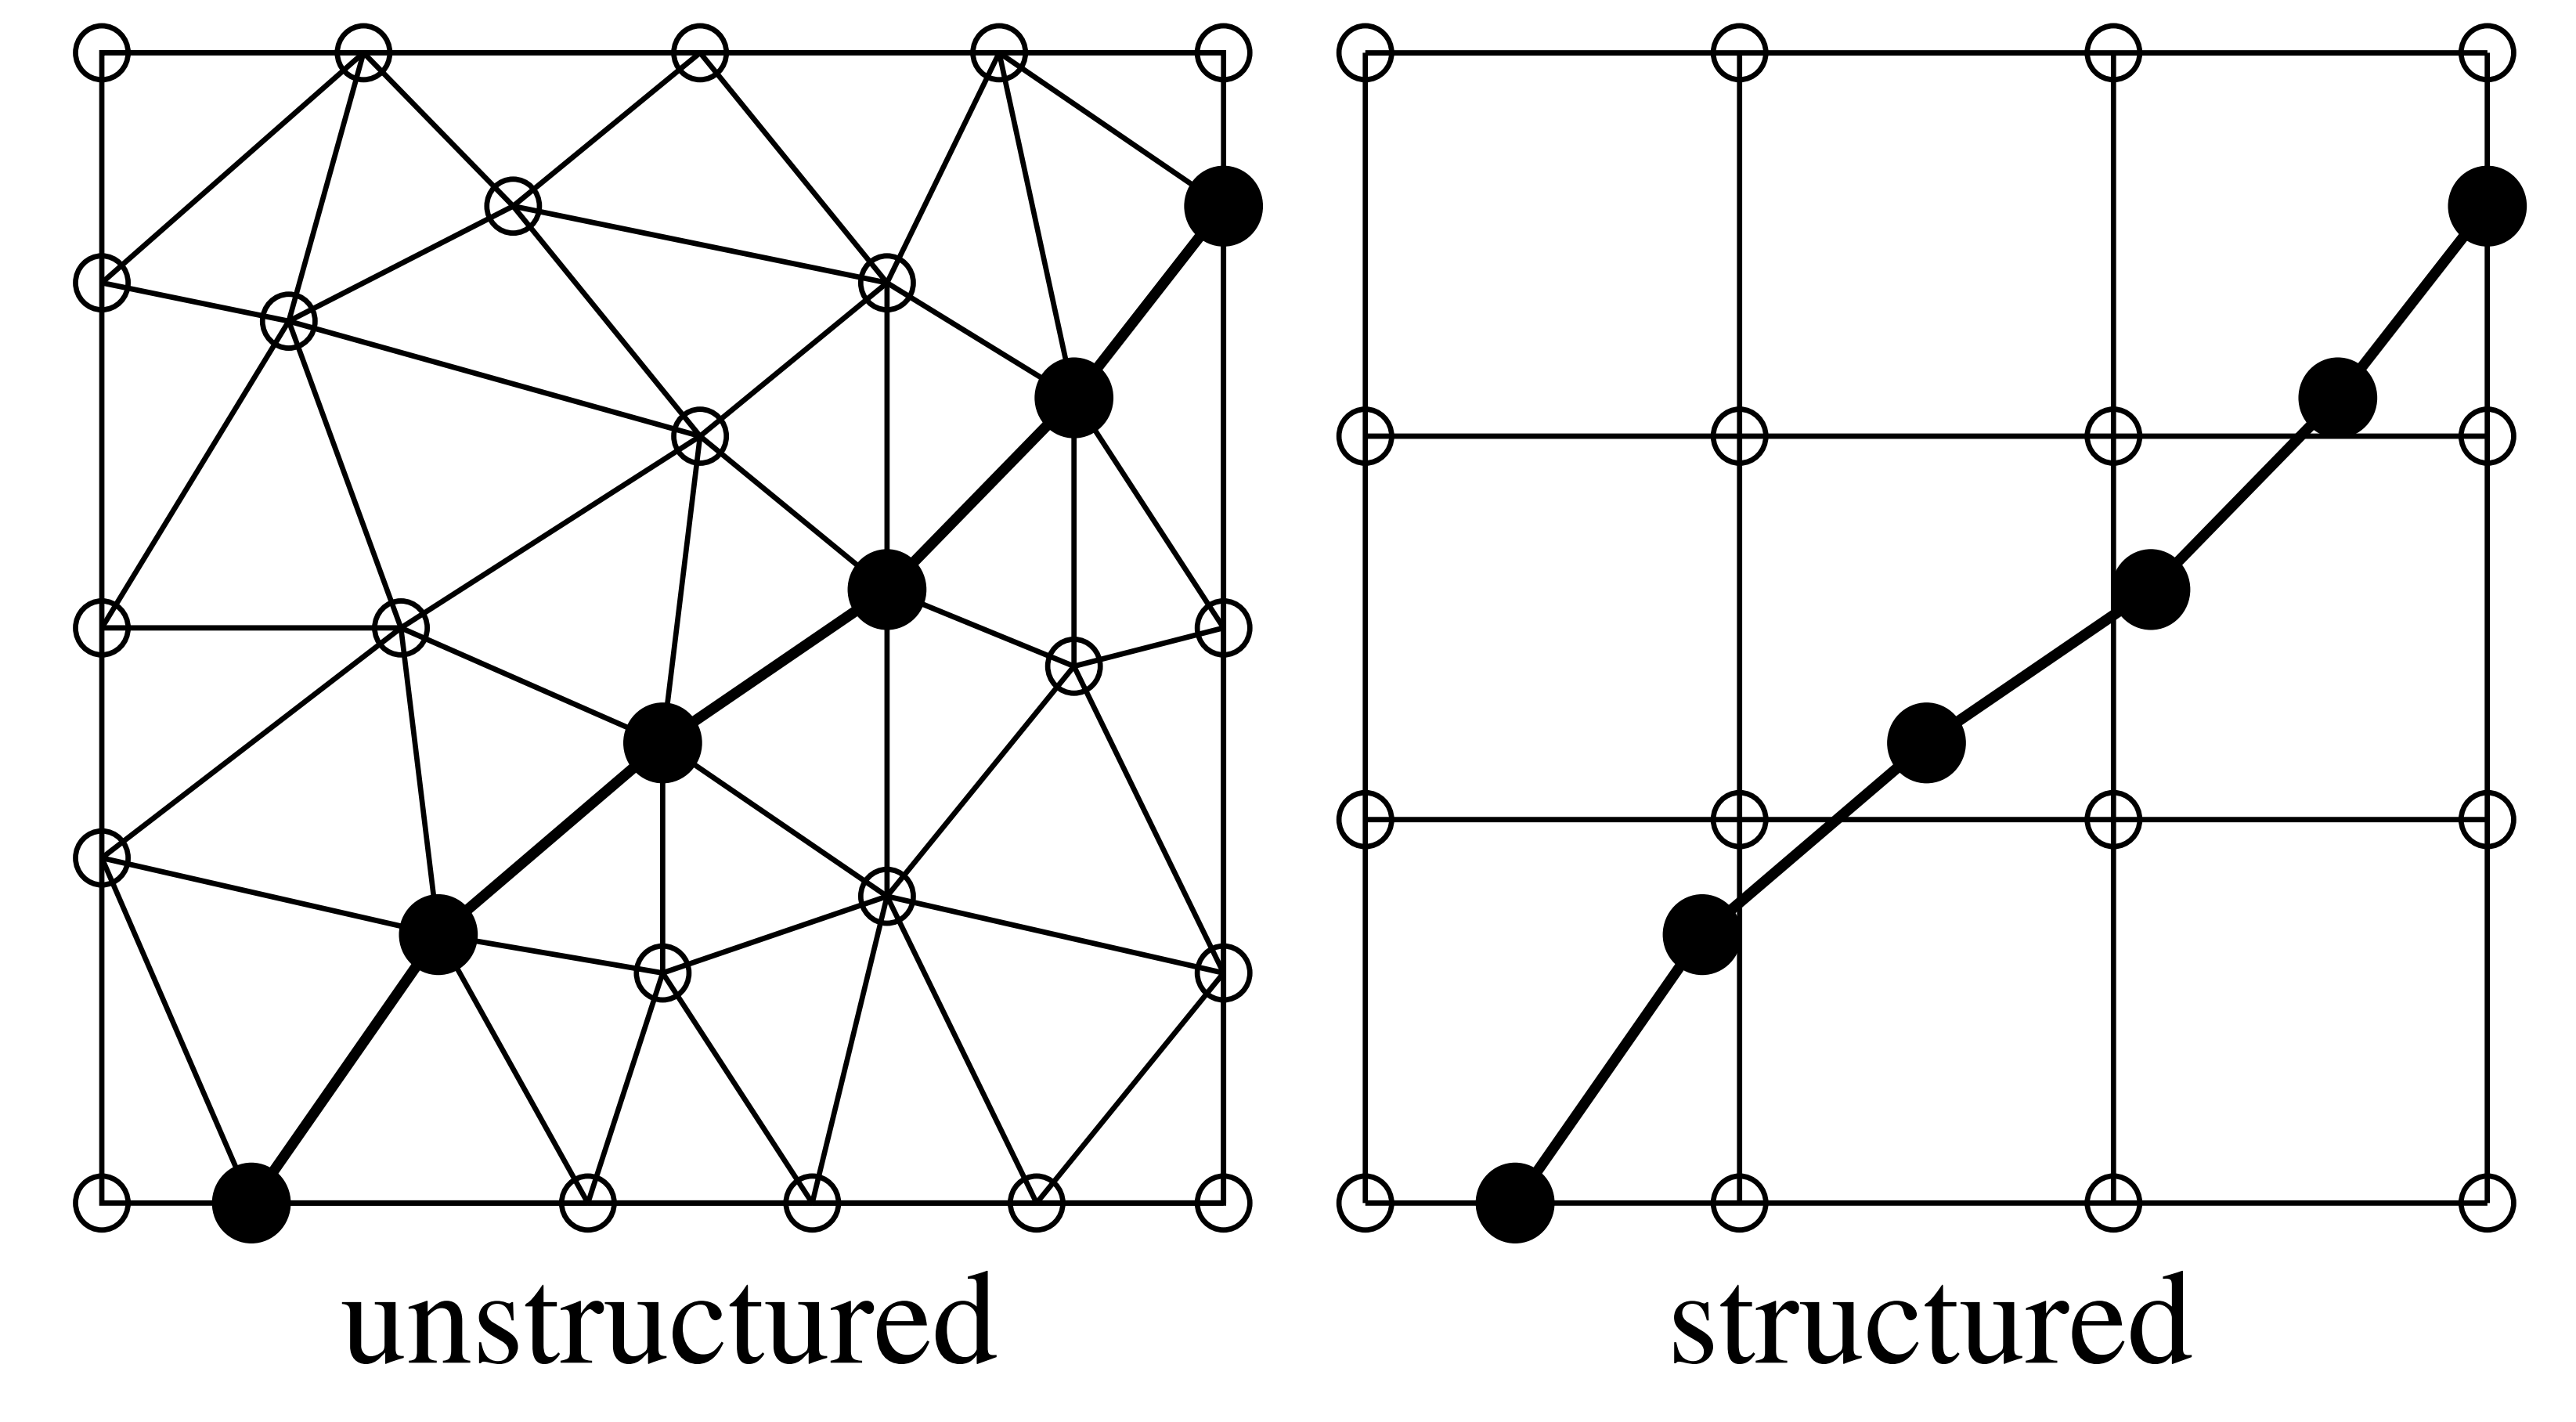
\includegraphics[width = 1 \textwidth]{obrazki/(un)structured_mesh.png} 
%\caption{blah}
\end{figure}
\end{center}
\end{frame}

\begin{frame}[fragile]\frametitle{Bounce Back Boundary Condition}
\begin{figure}[H]
\begin{center}
   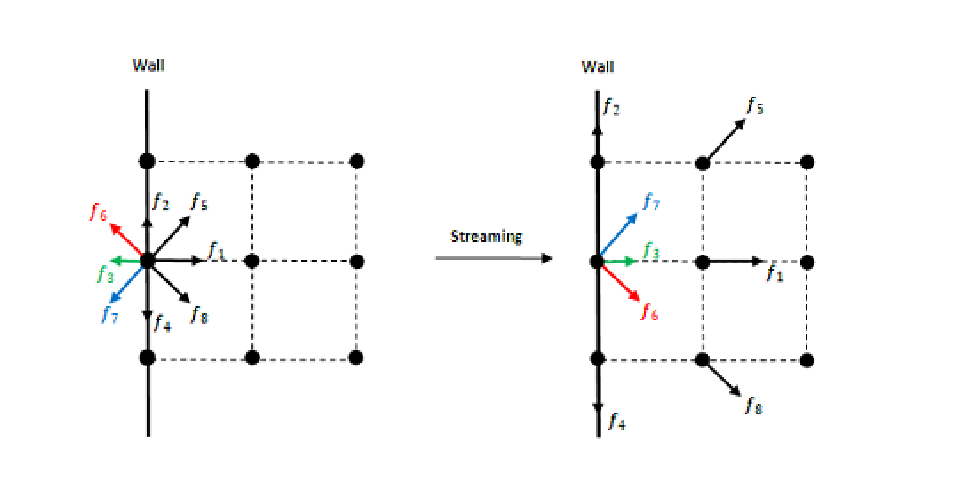
\includegraphics[width=0.8 \textwidth]{obrazki/bounceBack.png}  
   %\caption{On-grid bounce back  \autocite[p. 4] {Yuanxum}}
   %\label{fig:blabal}
 \end{center}
\end{figure}

\begin{align*} 
f_{\bar{i}}(\boldsymbol{x}_b,t + \Delta t) =  f_i (\boldsymbol{x}_b,t)
\end{align*}  
%Pseudocode:
%\begin{verbatim}
%for (int i = 0; i < N; ++i)
%    fOut[i] = fIn[oppositeIdx[i]];
%\end{verbatim}

\end{frame}

\begin{frame}\frametitle{Interpolated Bounce Back Boundary Condition}
%The Interpolated Bounce Back for curved boundaires has been proposed by \citeauthor{HamedBouzidi2001} \parencite{HamedBouzidi2001}.
It is assumed that during each streaming step, the population travels a distance $|\boldsymbol{e}_i| \Delta t$. 
%The walls are modelled by a half-way bounce back.
%As the name suggest, the algorithm employs an interpolation scheme between boundary node $\boldsymbol{x}_b$ and its neighbour,
\begin{figure}[H]
\begin{center}
   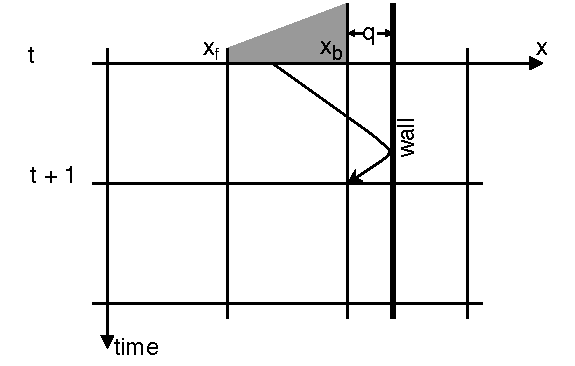
\includegraphics[width=0.6 \textwidth]{obrazki/IBB.pdf}  
   %\caption{On-grid bounce back  \autocite[p. 4] {Yuanxum}}
   %\label{fig:blabal}
 \end{center}
\end{figure}
\pause
\begin{align*}  
f_{\bar{i}}(\boldsymbol{x}_b,t + \Delta t)  &=
\left\{ 
	\begin{array}{ll}
				2q f_i^{*}(\boldsymbol{x}_b,t) + (1-2q)f_i^{*}(\boldsymbol{x}_f,t)
			  \hspace{3.0em} \text{for} \, q \in \left[0, 0.5 \right]  \vspace{1.5em} \\
			  %%			  
				\frac{1}{2q} f_i^{*}(\boldsymbol{x}_b,t) + \dfrac{2q-1}{2q} f_{\bar{i}}^{*}(\boldsymbol{x}_b,t)
			 \hspace{3.5em} \text{for} \,q \in \left( 0.5, 1 \right],
	\end{array} 
\right. \label{eq:IBB}
\end{align*}  
%where $q$ is the distance (along lattice link) between the boundary node and the actual boundary.
\end{frame}

\begin{frame}\frametitle{Dimensionless Numbers}
%Nusselt number represents the enhancement of heat transfer through a fluid as a result of convection relative to conduction across the same fluid layer. 
%In the simplest case, both convection and conduction heat flows are parallel to each other and to the surface normal of the boundary surface, and are all perpendicular to the mean fluid flow.
\begin{align*}
Nu = \frac{ h \Delta T}{k (\Delta T/D)}  = \frac{ h D}{k } 
\sim \dfrac{\text{convective heat transfer }}{\text{conductive heat transfer }}  
\end{align*}
%where h is the average heat convective transfer coefficient $[W/(m^2 K)]$, 
%while k stands for the thermal conductivity of the fluid $[W/(m K)]$. \\
%\hline

%Prandtl Number describes relative thickness of the momentum to thermal boundary layer:
\begin{align*}
Pr  = \frac{\nu}{\alpha}  = \frac{\nu \rho c_p}{k}
\sim  \dfrac{\text{molecular diffusivity of momentum}}{\text{molecular diffusivity of heat}}
\end{align*}
\begin{figure}[H]
 	\centering
		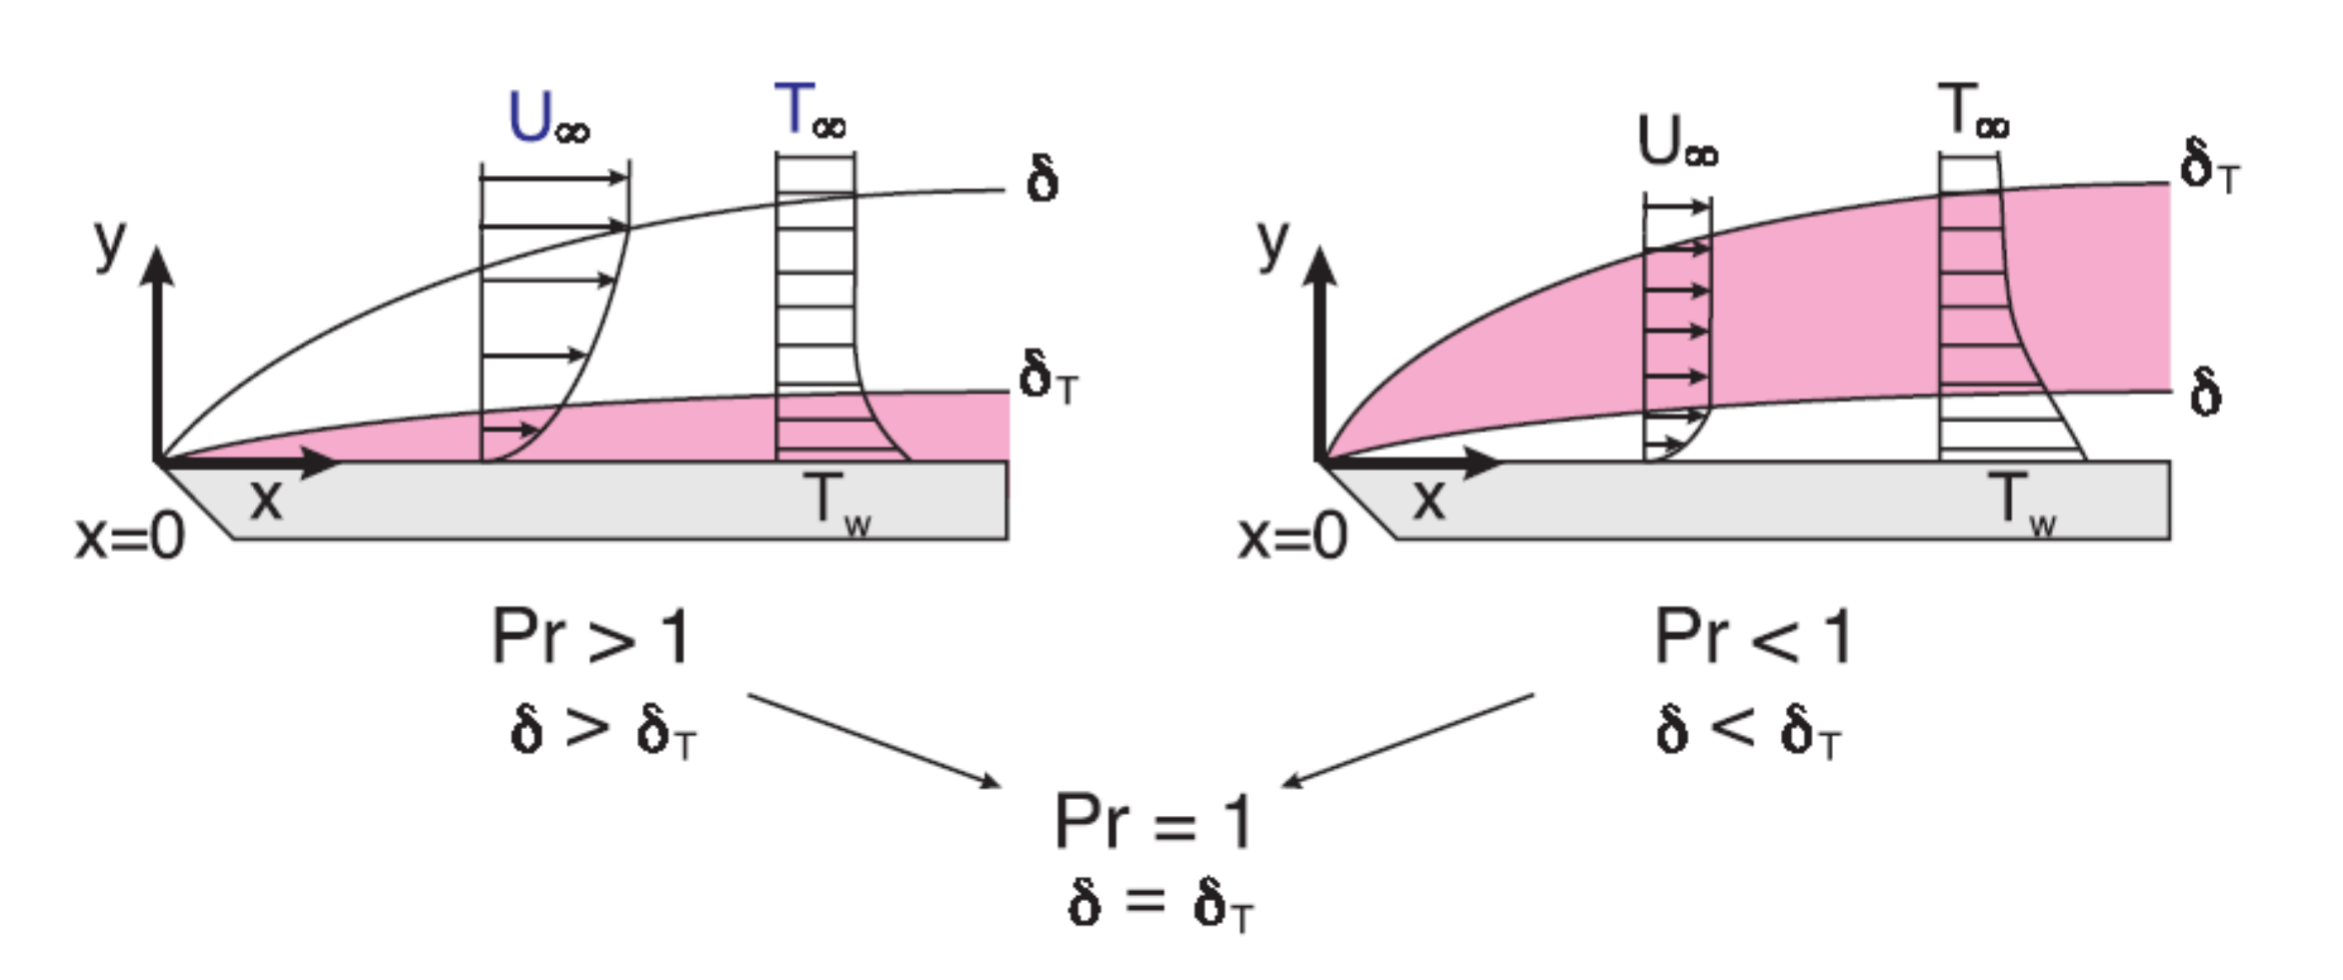
\includegraphics[width=1 \textwidth]{obrazki/thermalBL.png} 
	%\caption{Thermal and momentum boundary layer.}
	\label{fig:thermalBL}
\end{figure}
%For common fluids (e.g. oil), the Pr is usually high which means that heat diffuses much slower than the momentum and the thermal boundary layer is contained within the velocity boundary layer.
%In case of liquid metals, the Pr is low because heat diffuses much faster than momentum and the velocity boundary layer is fully contained within the thermal boundary layer. \\
\end{frame}
\subsection{Sample results}
\begin{frame}\frametitle{Scenarios}
\begin{table}[]
\resizebox{\textwidth}{!}{
\begin{tabular}{llllllllll}
Case-ID       & Lattice Size & Velocity set & Blockage Ratio & D   & U      & Pr   & Re & $\nu$   & $k$       \\  \hline \hline
Pr10$_{small}$    & 1000x150x3   & D3Q27Q27     & 1/5            & 30  & 0.01   & 10   & 10 & 3E-02 & 3E-03  \\
Pr10$_{medium}$   & 2000x300x3   & D3Q27Q27     & 1/5            & 60  & 0.005  & 10   & 10 & 3E-02 & 3E-03  \\
Pr10$_{large}$    & 4000x600x3   & D3Q27Q27     & 1/5            & 120 & 0.0025 & 10   & 10 & 3E-02 & 3E-03  \\
Pr100$_{small}$   & 1000x150x3   & D3Q27Q27     & 1/5            & 30  & 0.01   & 100  & 10 & 3E-02 & 3E-04  \\
Pr100$_{medium}$  & 2000x300x3   & D3Q27Q27     & 1/5            & 60  & 0.005  & 100  & 10 & 3E-02 & 3E-04  \\
Pr100$_{large}$   & 4000x600x3   & D3Q27Q27     & 1/5            & 120 & 0.0025 & 100  & 10 & 3E-02 & 3E-04  \\
Pr1000$_{small}$  & 1000x150x3   & D3Q27Q27     & 1/5            & 30  & 0.01   & 1000 & 10 & 3E-02 & 3E-05  \\
Pr1000$_{medium}$ & 2000x300x3   & D3Q27Q27     & 1/5            & 60  & 0.005  & 1000 & 10 & 3E-02 & 3E-05  \\
Pr1000$_{large}$  & 4000x600x3   & D3Q27Q27     & 1/5            & 120 & 0.0025 & 1000 & 10 & 3E-02 & 3E-05 
\end{tabular}
}
\caption{Case-ID: lookup table}
\label{tab:Case-ID_lookup_table}
\end{table}
\end{frame}

\begin{frame}\frametitle{Results}
\begin{table}[H]
\resizebox{\textwidth}{!}{
\begin{tabular}{llllll}
Case-ID       & $Nu_{CM\; HIGHER}^{1st\; order\; bc}$ & $Nu_{CM\; HIGHER}^{2nd\; order\; bc}$ & $Nu_{Cumulants}^{1st\; order\; bc}$ & $Nu_{Cumulants}^{2nd\; order\; bc}$ & $Nu_{FEM}$ \\  \hline \hline
Pr10$_{small}$    & 4.91                           & 4.81                           & 5.04                          & 4.83                          & 4.82    \\
Pr10$_{medium}$   & 4.86                           & 4.81                           & 4.92                          & 4.82                          & 4.82    \\
Pr10$_{large}$    & 4.83                           & 4.81                           & 4.87                          & 4.81                          & 4.82    \\
Pr100$_{small}$   & 10.66                          & 10.27                          & 14.50                         & 11.52                         & 10.1    \\
Pr100$_{medium}$  & 10.32                          & 10.13                          & 11.82                         & 10.36                         & 10.1    \\
Pr100$_{large}$   & 10.19                          & 10.08                          & 10.83                         & 10.13                         & 10.1    \\
Pr1000$_{small}$  & 27.09                          & 24.58                          & 94.31                         & 58.33                         & 21.43   \\
Pr1000$_{medium}$ & 22.73                          & 21.84                          & 53.97                         & 34.19                         & 21.43   \\
Pr1000$_{large}$  & 21.84                          & 21.37                          & 34.04                         & 24.56                         & 21.43  
\end{tabular}
}
\caption{Influence of kernel and BC on Nu number. \\
${1st\; order\; bc}$ = BB (hydrodynamics) + EQ (thermodynamics) \\
${2nd\; order\; bc}$ = IBB (hydrodynamics) + IABB (thermodynamics)
}

\label{tab:my-table}
\end{table}
\end{frame}


%\begin{frame} % \frametitle{Results 2 }
%
%\begin{table}[H]
%\resizebox{\textwidth}{!}{
%\begin{tabular}{llllll}
%Case-ID       & $Nu_{CM\; HIGHER}^{1st\; order\; bc}$ & $Nu_{CM\; HIGHER}^{2nd\; order\; bc}$ & $Nu_{Cumulants}^{1st\; order\; bc}$ & $Nu_{Cumulants}^{2nd\; order\; bc}$ & $Nu_{FEM}$ \\  \hline \hline
%Pr10$_{small}$    & 4.91                           & 4.81                           & 5.04                          & 4.83                          & 4.82    \\
%Pr10$_{medium}$   & 4.86                           & 4.81                           & 4.92                          & 4.82                          & 4.82    \\
%Pr10$_{large}$    & 4.83                           & 4.81                           & 4.87                          & 4.81                          & 4.82    \\
%Pr100$_{small}$   & 10.66                          & 10.27                          & 14.50                         & 11.52                         & 10.1    \\
%Pr100$_{medium}$  & 10.32                          & 10.13                          & 11.82                         & 10.36                         & 10.1    \\
%Pr100$_{large}$   & 10.19                          & 10.08                          & 10.83                         & 10.13                         & 10.1    \\
%Pr1000$_{small}$  & 27.09                          & 24.58                          & 94.31                         & 58.33                         & 21.43   \\
%Pr1000$_{medium}$ & 22.73                          & 21.84                          & 53.97                         & 34.19                         & 21.43   \\
%Pr1000$_{large}$  & 21.84                          & 21.37                          & 34.04                         & 24.56                         & 21.43  
%\end{tabular}
%}
%\caption{Influence of kernel and BC on Nu number. \\
%%${1st\; order\; bc}$ = BB (hydrodynamics) + EQ (thermodynamics) \\
%%${2nd\; order\; bc}$ = IBB (hydrodynamics) + IABB (thermodynamics)
%}
%
%\label{tab:my-table}
%\end{table}
%
%\begin{table}[]
%\resizebox{\textwidth}{!}{
%\begin{tabular}{llllllllll}
%Case-ID       & Lattice Size & Velocity set & Blockage Ratio & D   & U      & Pr   & Re & $\nu$   & $k$       \\  \hline \hline
%Pr10$_{small}$    & 1000x150x3   & D3Q27Q27     & 1/5            & 30  & 0.01   & 10   & 10 & 3E-02 & 3E-03  \\
%Pr10$_{medium}$   & 2000x300x3   & D3Q27Q27     & 1/5            & 60  & 0.005  & 10   & 10 & 3E-02 & 3E-03  \\
%Pr10$_{large}$    & 4000x600x3   & D3Q27Q27     & 1/5            & 120 & 0.0025 & 10   & 10 & 3E-02 & 3E-03  \\
%Pr100$_{small}$   & 1000x150x3   & D3Q27Q27     & 1/5            & 30  & 0.01   & 100  & 10 & 3E-02 & 3E-04  \\
%Pr100$_{medium}$  & 2000x300x3   & D3Q27Q27     & 1/5            & 60  & 0.005  & 100  & 10 & 3E-02 & 3E-04  \\
%Pr100$_{large}$   & 4000x600x3   & D3Q27Q27     & 1/5            & 120 & 0.0025 & 100  & 10 & 3E-02 & 3E-04  \\
%Pr1000$_{small}$  & 1000x150x3   & D3Q27Q27     & 1/5            & 30  & 0.01   & 1000 & 10 & 3E-02 & 3E-05  \\
%Pr1000$_{medium}$ & 2000x300x3   & D3Q27Q27     & 1/5            & 60  & 0.005  & 1000 & 10 & 3E-02 & 3E-05  \\
%Pr1000$_{large}$  & 4000x600x3   & D3Q27Q27     & 1/5            & 120 & 0.0025 & 1000 & 10 & 3E-02 & 3E-05 
%\end{tabular}
%}
%\caption{Case-ID: lookup table}
%\label{tab:Case-ID_lookup_table}
%\end{table}
%\end{frame}

\subsection{Memory requirements}
%\begin{frame}\frametitle{Memory requirements}
%\begin{table}[]
%\centering
%\resizebox{\textwidth}{!}{%
%\begin{tabular}{lll}
%edge length {[}lu{]} & No nodes {[}-{]} & mem allocation {[}GB{]} \\ \hline
%32                   & 3.28E+04         & 0.03                    \\
%64                   & 2.62E+05         & 0.26                    \\
%128                  & 2.10E+06         & 2.05                    \\
%256                  & 1.68E+07         & 16.37                   \\
%512                  & 1.34E+08         & 131.00                  \\
%1024                 & 1.07E+09         & 1,047.97               
%\end{tabular}%
%}
%\caption{}
%\label{tab:my-table}
%\end{table}
%\end{frame}


\begin{frame}\frametitle{Memory requirements}

\begin{table}[]
\centering
%\resizebox{0.8\textwidth}{!}{%
\begin{tabular}{l|lll}
                & No {[}-{]} & {[}double{]} & {[}Bytes{]} \\ \hline
DF              & 2x27       & 54           & 432         \\
DF temp         & 2x27       & 54           & 432         \\
q               & 2x27       & 13.5         & 108         \\
flag            & 1          & 0.5          & 4           \\
                &            &              &             \\
memory per node &            & 122          & 976        
\end{tabular}%
%}
\caption{Theoretical memory requirements for: \newline 3D, DDF model with interpolated BC}
%\label{tab:my-table}
\end{table}

\end{frame}


\begin{frame}\frametitle{Memory requirements}
\begin{figure}
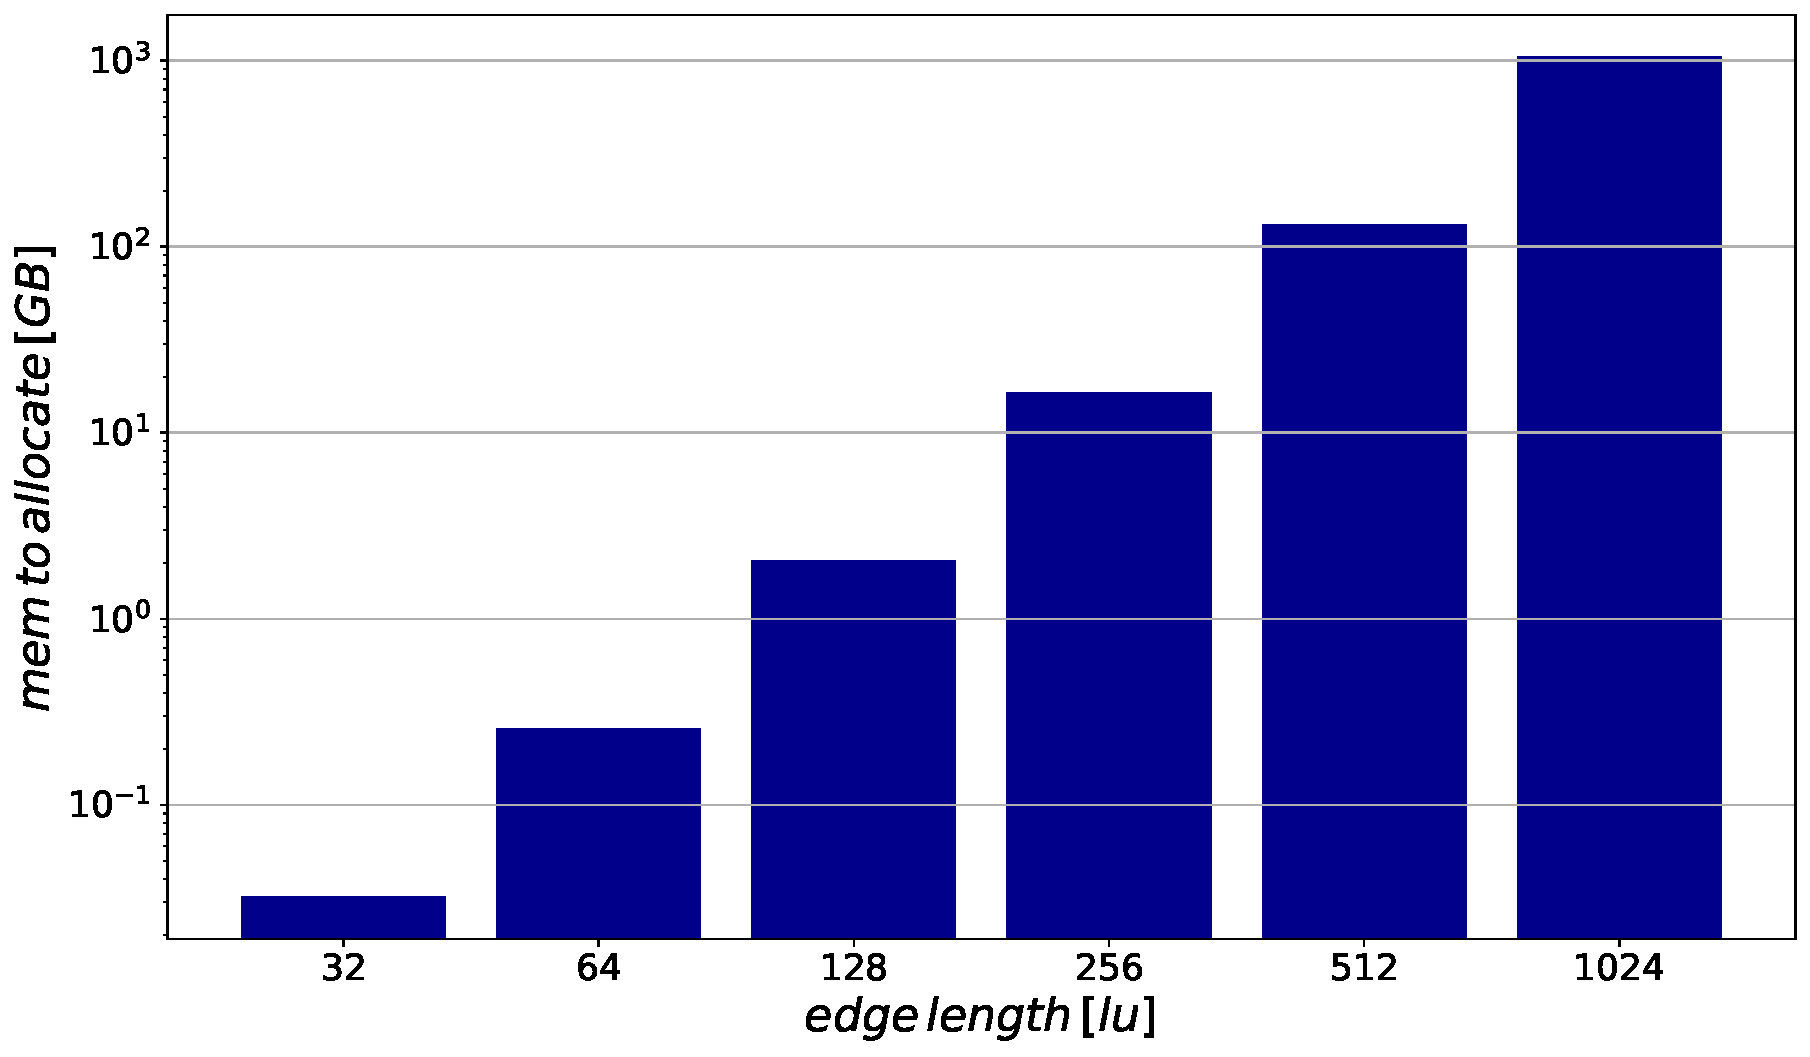
\includegraphics[width = 1 \textwidth]{obrazki/log_mem_req.pdf} 
\caption{Theoretical memory requirements for: \newline 3D, DDF model with interpolated BC}
\end{figure}
\end{frame}


\begin{frame}\frametitle{Memory requirements}
\textbf{Q:} Does the high memory requirement limits applicability of LBM? \\ \vspace{1.5em}
\pause
Not necassary. Similar problems occur in other CFD methods like VOF, FEM, FD.
The common solutions are:
\begin{enumerate}
\item Mesh refinement. 
\item Chimera (overlapping) mesh. 
\end{enumerate}
\end{frame}

\begin{frame}\frametitle{Questions?}
\begin{center}
%{\huge ? }
\begin{figure}
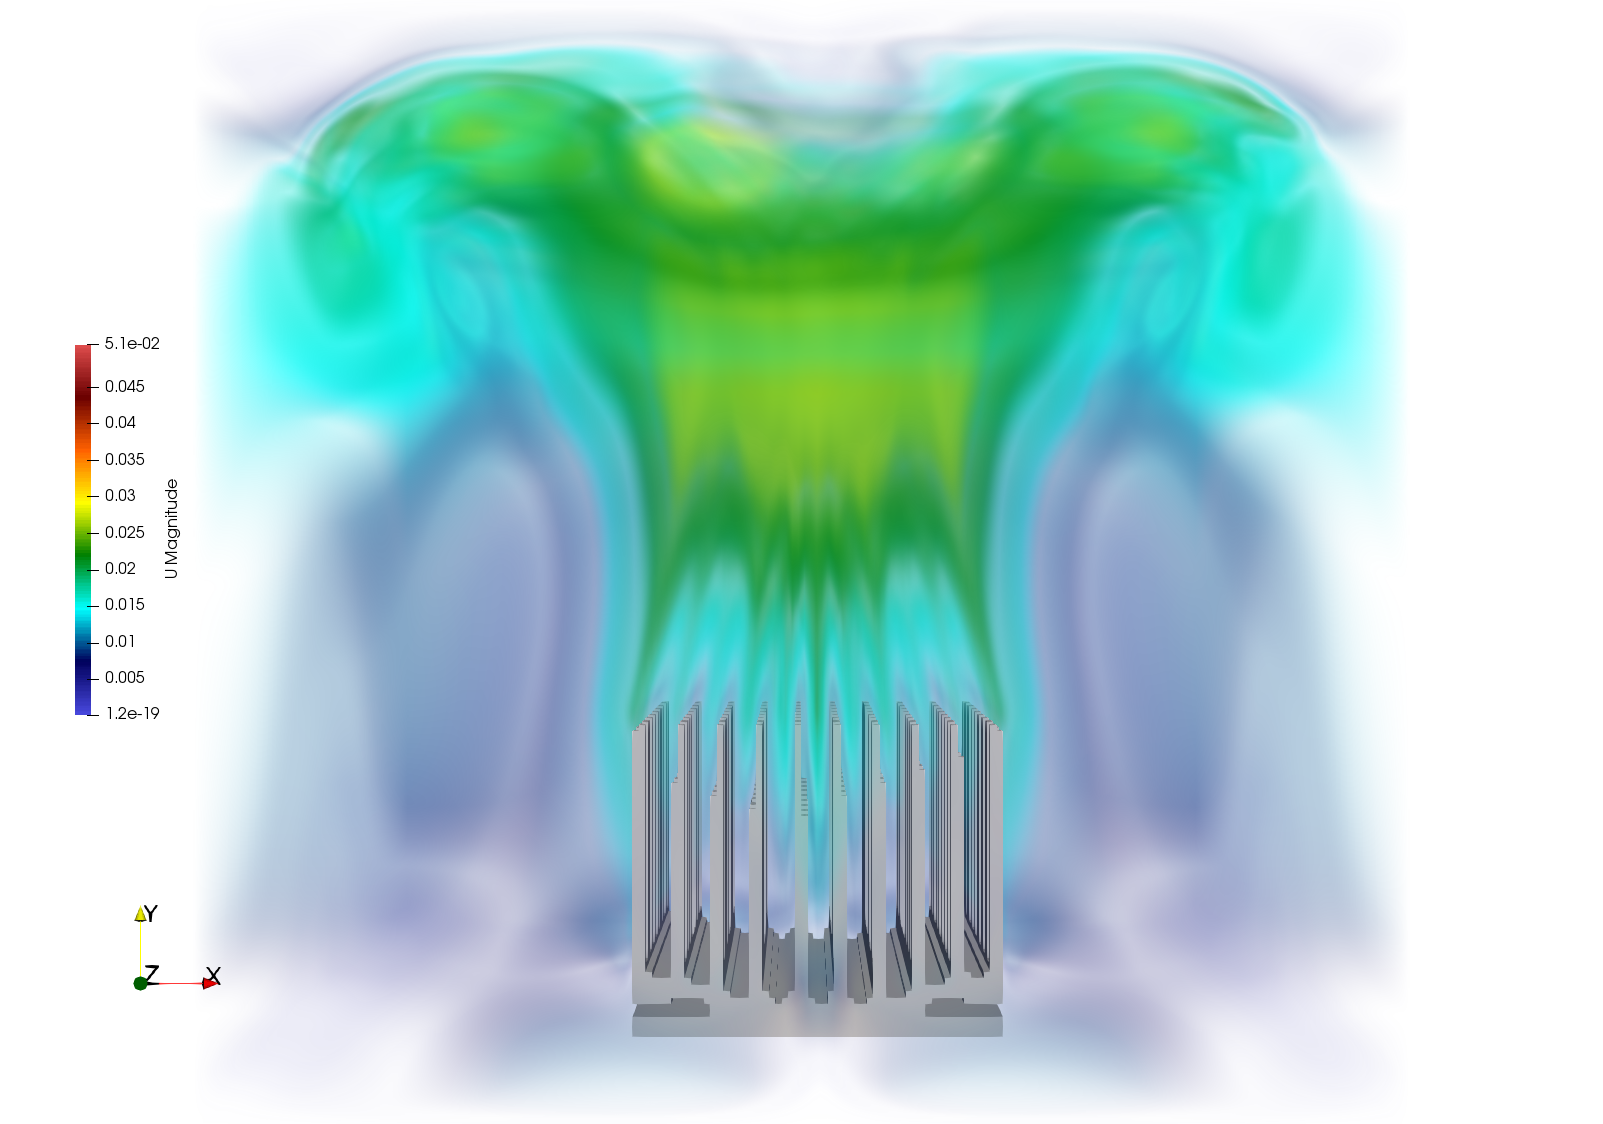
\includegraphics[width = 1 \textwidth]{obrazki/u_volume2.png} 
%\caption{blah}
\end{figure}
\end{center}
\end{frame}

%\begin{frame}[t,allowframebreaks]
%\frametitle{References}
%%\bibliography{<bibfile>}
%\printbibliography[title=References]
%%\nocite {TCLB}
%\end{frame}


\appendix

%\begin{frame}{Backup slied}
%    Something to cover your back. This slides are not being numbered nor included in progress bar (thin line below title bar)
%\end{frame}


\end{document}
